\documentclass[a4paper,12pt]{article}
\usepackage{caption}
\usepackage{subcaption}
\usepackage{float}
\usepackage{dsfont}
\usepackage[T1]{fontenc}
\usepackage[italian]{babel}
\usepackage[utf8]{inputenc}
\input funzioni.sty
\input funzioni2.sty
\floatstyle{ruled}
\usepackage{hyperref}
\usepackage{graphicx}
\usepackage{amsmath}
\usepackage{amssymb}
\usepackage[width=125mm]{caption}
\usepackage{amsthm}
\usepackage{algorithm2e}
\usepackage{algpseudocode}
\usepackage{empheq}
\usepackage{tikz}
\usepackage{cancel}

% Dimensione della pagina
\setlength{\oddsidemargin}{.3in}  % Distance from the left edge -1 inch 
\setlength{\textwidth}{145mm}     % Normal width of the text
\setlength{\topmargin}{.25in}     % Distance from top to PAGE'S HEAD -1 inch
\setlength{\textheight}{225mm}    % Height of the body of page
\setlength{\headheight}{0mm}      % Height of a box containing the head
\setlength{\parskip}{0.5mm}         % Extra vertical space before a paragraph
\setlength{\parindent}{9mm}       % Width of the indentation 
\linespread{1.12}                 % Line spacing        
\renewcommand{\floatpagefraction}{.9}

\newtheorem{Teorema}{Teorema}

\begin{document}
\title{\bf \Huge Stuttura della Materia 1 e 2 }
\maketitle

\newpage
\tableofcontents
\newpage

%----------------------------------------------------------------------------
\section{Particella in Campo Centrale}
%----------------------------------------------------------------------------
L'operatore che descrive il fenomeno sarà dato dalla parte cinetica e dalla parte di potenziale, che dipenderà in un qualche modo da $r$. In particolare 
\newl{\op{H} = \frac{1}{2m}\sum\op{p} ^2 + U\left(\sqrt{\sum x^2}\right).}
Definendo l'operatore \textit{Momento Angolare Orbitale} come
\newl{\op{L} _i = \varepsilon_{ijk}\op{x} _j \op{p} _k}
che in modo esplicito si scrive come
\newl{\op{L} _x = y p_z - z p_y \;\; ; \;\;  \op{L} _y = zp_x - xp_z \;\; ; \;\; \op{L} _z = xp_y - yp_x}
\begin{Teorema}
	Ogni operatore che può essere scritto nella forma $\ps{\op{v_1} }{\op{v_2} } $ commuta con $\op{L} $.
\end{Teorema}
\begin{proof}
\newl{\left[\op{L}, \op{v} _1\cdot \op{v} _2\right] &=& \sum_k \left[\op{L} _h, \op{v} _{1k} \right]\op{v} _{2k} + \sum_k \op{v} _{1k} \left[\op{L} _h, \op{v} _{2k} \right] = i\hbar\varepsilon_{hkl}\op{v} _{1l} \op{v} _{2k} + i\hbar\varepsilon_{hkl} \op{v} _{1k} \op{v} _{2l} =\nonumber \\ &=&i\hbar(\varepsilon_hkl + \varepsilon_{khl}) \op{v} _{1k} \op{v} _{2k} = 0 }
\end{proof}
In virtù di questo, si ottiene il risultato notevole
\newl{[\op{L} , \op{p} ^2] \;\; , \;\; [\op{L} , \op{v} ^2]}
Se due operatori essenzialmente autoaggiunti commutano tra loro, allora l'autospazio di uno è l'autospazio dell'altro. \footnote{Perlomeno... credo che dovrebbe essere così...}. In questo modo è possibile notare che $\op{L} $ commuta con l'Hamiltoniana di campo centrale $\op{H} = k \op{p} ^2 + f(\op{r} \cdot \op{r} )$
\newl{[\op{L} , \op{H} ] = [\op{L}, \op{p} ^2] + [\op{L} , f(\op{r} \cdot \op{r} )] = 0.}
Per sfuttare il lemma di Shur, si costruisce per praticità l'operatore $\op{L} ^2$ definito come
\newl{\op{L} \cdot \op{L} = \op{L} _x^2 + \op{L} _y^2 + \op{L} _z^2 = \op{L} ^2 .}
$\op{L} ^2$ commuta con $\op{L} _z$, quindi posso pensare di decomporre lo spazio di Hilbert negli autospazi di $\op{L} ^2$ e $\op{L} _z$. Seguendo la simmetria del problema riscrivo l'operatore $\op{L} ^2$ in coordinate sferiche
\newl{\op{L} ^2 = -\hbar^2 \left(\frac{1}{\sin\vartheta} \frac{\partial}{\partial\theta} \sin \vartheta \frac{\partial}{\partial \vartheta} + \frac{1}{\sin^2 \vartheta} \frac{\partial^2}{\partial \varphi ^2}\right) }
insieme all'operatore laplaciano
\newl{-\frac{\hbar^2}{2m}\Delta_2 = -\frac{\hbar^2}{2m}\frac{1}{r^2}\frac{\partial}{\partial r} r^2 \frac{\partial}{\partial r} + \frac{1}{2m r^2} \op{L} ^2 }
\subsection{L'autospazio di $L_z$}
Sfruttando le simmetrie del problema, posso trovare l'autospazio di $L_z$. Dato che commuta con $L^2$, che a sua volta commuta con l'Hamiltoniano, trovare l'autospazio di $L_z$ equivale trovare uno spazio in cui posso andare a cercare le autofunzioni di $\op{H} $. Presa una $f(r,\vartheta,\varphi)\in L^2(\R^3)$ continua e periodica nella variabile $\varphi$. Risolvo il problema agli autovalori dell'operatore $L_z$ che è definito come $L_z=-i\hbar \partial/\partial\varphi$
\newl{-i\hbar\frac{\partial}{\partial \varphi} f(r,\vartheta, \varphi) = \lambda f(r,\vartheta, \varphi).}
Fissando $r$ e $\vartheta$ ottengo un'equazione differenziale nella variabile $\varphi$ 
\newl{\frac{\partial}{\partial \varphi} \frac{f}{f(\varphi)} = \frac{i\lambda}{\hbar}.}
La soluzione è immediata
\newl{\log( f(\varphi) ) = \frac{i\lambda}{\hbar} \varphi \;\;\implicaa\;\; f(\varphi) = A\cdot e^{\frac{i\lambda}{\hbar} \varphi}   .}
Le autofunzioni di $L_z$ sono quindi del tipo
\newl{f(r,\vartheta,\varphi) = A(r,\vartheta) e^{\frac{i\lambda}{\hbar}\varphi} .}
Gli autovalori li ottengo imponendo le condizioni sull'angolo $\varphi$,
\newl{0\leq\varphi\leq 2\pi \;\;\implicaa \;\; e^{\frac{i\lambda 2\pi}{\hbar}}=1 }
la condizione su $\lambda$ diventa quindi
\newl{\lambda = \hbar m\;\;\;\;\; m \in N .}
Concludendo l'autospazio di $L_z$ è
\newl{S_m=\left\lbrace\frac{A(r,\vartheta)}{\sqrt{2\pi}}e^{im\varphi}\right\rbrace. }
Queste autofunzioni generano tutto lo spazio di Hilber e costuituiscono un s.o.n.c.
La somma ortogonale di tutti gli spazi $S_m$ genera tutto $L^2 (\R^3 )$ 
\newl{\oplus \sum_mS_m = L^2 (\R^3).}
In questo modo vale che $\forall f(r,\vartheta,\varphi) \in L^2(\R^3)$ è possibile scriverla sviluppata sulla base di $S_m$
\newl{f(r,\vartheta,\varphi) = \sum_{-\infty}^{+\infty} \frac{A(r,\vartheta)}{\sqrt{2\pi}} e^{im\varphi}}
dove le $A(r,\vartheta)$ sono funzioni t.c. $\int_{-\infty}^{+\infty}r^2\,dr\int_0^{2\pi}\sin\vartheta\abs{A(r,\vartheta)} \,d\vartheta<\infty$. Antitrasformando è possibile ricavare in modo formale le $A(r,\vartheta)$
\newl{A(r,\vartheta) = \int_0 ^{2\pi} \frac{1}{\sqrt{2\pi}} e^{-im\varphi'} f(r,\vartheta,\varphi') \,d\varphi'.}
La misura che faccio sull'osservabile $f$ può quindi essere vista come una proiezione dalle funzioni di $L^2(\R^3)$ sullo spazio di $L_z$. Questo viene definito come \textit{misura a valore di proiettore} e l'operatore che ne descrive il funzionamento è dato da
\newl{(\op{\mathds E} _{S_m}^{L_z} f)(r,\vartheta,\varphi) = \frac{A_m(r,\vartheta)}{\sqrt{2\pi}} e^{im\varphi} = \frac{1}{\sqrt{2\pi}}\int_0 ^{2\pi} e^{-im\varphi'} f(r,\vartheta,\varphi') \,d\varphi' .}
Se $f$ è un autostato di $L_z$ la sua rappresentazione è
\newl{(\op{L} _z f)(r,\vartheta,\varphi)= \sum_{m=-\infty}^{+\infty} \hbar m A(r,\vartheta) \frac{e^{im\varphi}}{\sqrt{2\pi}} = \sum_{m=-\infty}^{+\infty} \hbar m (\op{\mathds E} _{S_m}^{L_z} f)(r,\vartheta,\varphi)  }


\section{Fisica della Materia e della Radiazione}
Si definisce \textbf{Materia Condensata} un insieme di particelle interagenti. In funzione del numero di particelle, possiamo avere strutture diverse.
\begin{itemize}
	\item Nanostrutture $[\text{nm}]$ = caratterizzate da poche particelle interangeti, sul centinaio $(<10^3)$. Ovviamente avendo pochi atomi si hanno sttrutture molto piccole;
	\item Mesostrutture $[\mu m]$ = caratterizate da un numero di particelle di $\sim  10^4$;
	\item Strutture macroscopiche $[mm]$ = sono caratterizzate da un $N_A$ di particelle interagenti.
\end{itemize}
Lo scopo del fisico è quello di costruire modelli fisici partendo dall'osservazione. L'osservazione di un determinato fenomeno induce una domanda alla quale si cerca di rispondere attraverso la costruzione di un modello fisico. Davanti alla necessità di costruire un modello nasce il grande dilemma: quando usare un modello classico? Quando uno quantistico? La risposta varia di caso in caso. Per esempio la descrizione di una particella intesa come pacchetto d'onda, può cambiare molto in funzione al problema che studiamo. Se ho sovrapposizione ho effetti quantistici che non posso trascurare (per esempio l'interazione di scambio).

Se considero i pacchetti d'onda non sovrapposti in cui $p\gg (\Delta p)$ e  $V/N \gg (\Delta r)^3$ allora posso usare un modello classico. Usando la lunghezza termica di De Broglie
\newl{\lambda_D=\frac{h}{p}=\frac{h}{\sqrt{2mE_C}} = \left(\frac{h^2}{3mK_BT}\right)^{\frac{1}{2}}}
posso verificare che 
\newl{\frac{N}{V}\lambda_D^3 = \frac{N}{V}\left(\frac{h^2}{3mK_BT}\right)^{\frac{3}{2}}\ll 1.}
La stessa considerazione è possibile farla partendo dal principio di indeterminazione di Heisenberg scritto nella ususale forma
\newl{\Delta r \cdot \Delta p \geq h.}
Possiamo quinid ricavare la stessa cosa di prima partendo da
\newl{\frac{V}{N}p^3 \gg (\Delta r) \cdot (\Delta p) \geq h^3}
sapendo che $p=(3mK_BT)^{\frac{1}{2}}$ riottengo 
\newl{\frac{N}{V}\left(\frac{h^2}{3mK_BT}\right)^{\frac{3}{2}}\ll 1.}
Un sistema può quindi essere modellizzato in modo classico per \textbf{densità} molto alte, \textbf{temperature} molto basse e \textbf{masse} molto piccole. Alcuni esempi sono dati da
\begin{itemize}
	\item Gas di idrogeno $[T\sim 0.26 K]$ sotto questa temperatura può essere modellizzato con le leggi classiche della cinetica dei gas;
	\item Elettroni di conduzione $[T \sim 1.8\cdot 10^5K]$ per modellizzare questo sistema ho necessità di usare modelli quantistici;
	\item Molti fotoni $(>10^3)$ ho il campo elettromagnetico classico, quindi le equazioni di Maxwell;
	\item Pochi fotoni $(<10)$ ho la QED (Quantum Elettro Dynamic).
\end{itemize}

\section{Richiamo sui solidi}
La materia che si presenta sotto il suo stato di \textit{solido} ha la caratteristica di essere completamente ordinata, gode di simmetria per alcuni angoli particolari e ci sono delle periodicità nella struttura. Sistemi solidi amorfi si conoscono per 0D (così detti \textit{quantum dot} ), 1D e 2D (così detti \textit{quantum well} come per esempio il grafene). Oltre ai sistemi amorfi ci sono i \textit{Quasi Cristalli}. Sono caratterizzati dall'avere simmetrie miste, per esempio parti con celle penatgonali miste a parte con simmetria sferica. Per osservare come la materia è aggregata, quali simmetrie sono presenti ed eventuali correlazioni le osservazioni che si possono fare riguardano le figure di difrazione costruite facendo diffrangere radiazioni differenti. In funzione al passo del reticolo\footnote{E' vera questa cosa? C'è effettivamente una correlazione tra campione che voglio studiare e la relazione che scelgo per studiarlo? Credo proprio di sì.} si possono studiare diferse immagini di diffrazione costruite per esempio con raggi X($1 KeV \sim 10KeV$), con diffrazione di neutroni ($0,1 eV\sim 1 eV$) oppure strutture superficiali, diffrazione di elettroni ($100 eV$). A temperature prossime a quelle dell'ambiente ($T\sim 300K$) i neutroni hanno un loro momento magnetico. In questo modo, vedendo l'interazione tra i netroni e la mataria posso farmi un'idea sulle sue proprietà magretiche. Quindi, in conclusione, se devo studiare le proprietà magnetiche della materia uso neutroni a temperatura prossima a quella ambientale. 
\subsection{Reticolo di Bravais}
Un reticolo generico è possibile definirlo come 
\newl{\vet{R} = n_1 \vet{a} _2   + n_2 \vet{a} _2 + n_3 \vet{a} _3} 
in cui però i vettori $\vet{a} _i$ non devono essere complanari. Il reticolo a nido d'ape, per esempio, non è un reticolo di Bravais perchè non è un gruppo puntuale.
\section{Teoria elementare della diffrazione}
Ho un oggetto da studiare come in fig.$\ref{Diff:1}$.
\begin{figure}
	\centering
	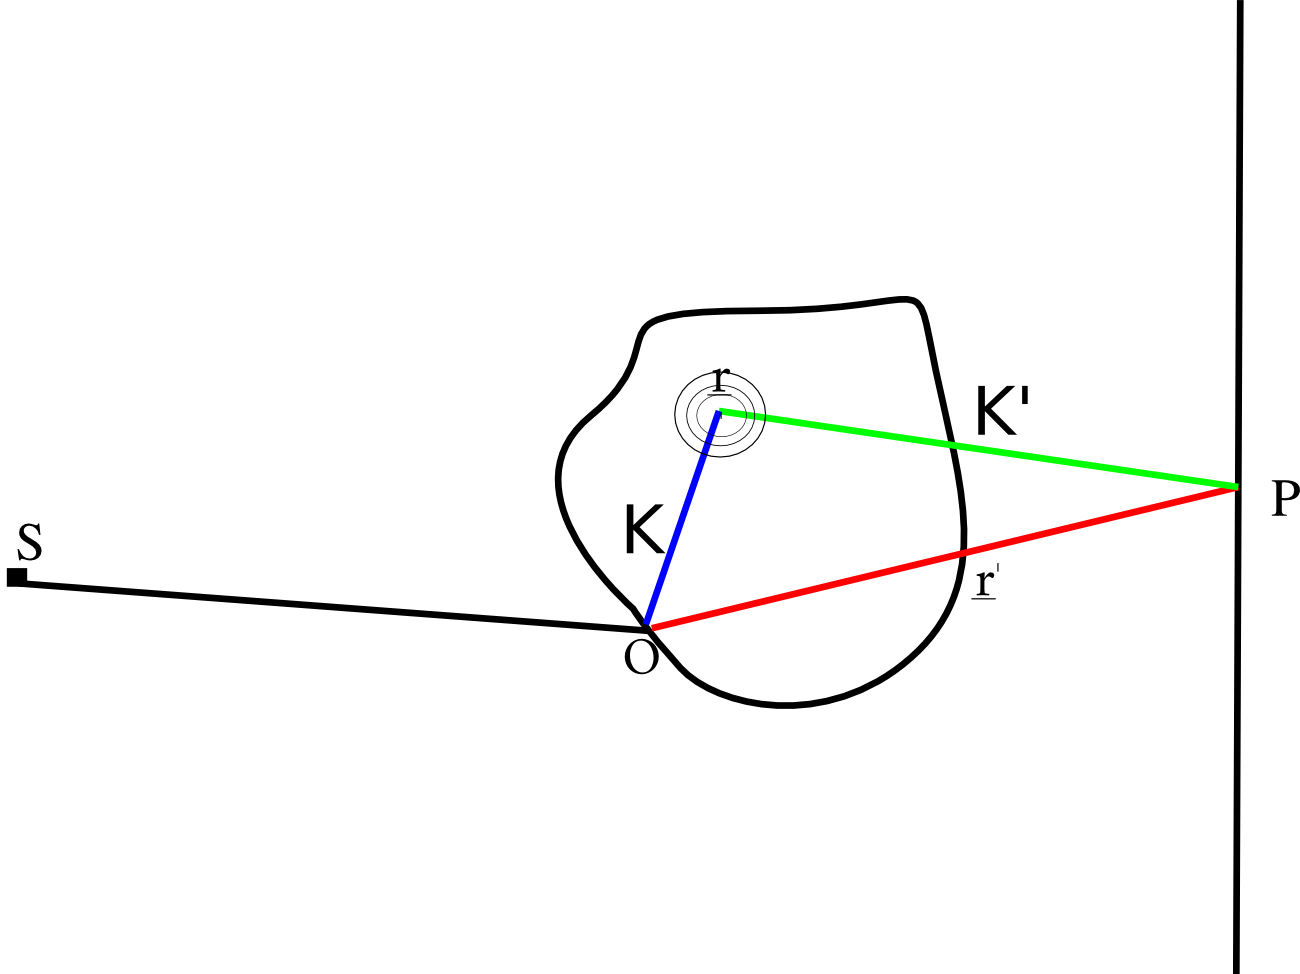
\includegraphics[width=120mm,angle=0,clip=]{IMG/Diff.png}
	\caption{Prova}
	\label{Diff:1}
\end{figure}
Supponendo $S$ una sorgente puntiforme e continua, la radiazione colpisce l'oggetto nel punto $\vec{r} $ diventando una sorgente di onde sferiche. Lo schermo si trova molto distante dall'oggetto colpito dalla radiazione, quindi $|r'| \gg |r|$. La sorgente manda onde piane quindi
\newl{A(r)=A_Se^{i[k(r+R)-\omega t]}}
Voglio evitare lo scattering multiplo. Singola interazione per ogni particella. L'onda interagisce con l'oggetto nel punto $r$ generando onde sferiche che raggiungeranno lo schermo e verranno viste nel punto $P$. Le onde difratte avranno come vettore d'onda $k'$. Quello che vedo nel punto $P$ sarà proporzionale a
\newl{A_P(r)=\int d^3r A(r)\rho(r)\left(\frac{e^{ik\cdot(r'-r)}}{|r'-r|}\right)}
dove $\rho(r)$ è la densità elettronica nel punto di interazione. Sviluppando l'espressione del potenziale nel punto $P$ e raggruppando tutti i termini indipendenti da $r$ ottengo
\newl{A_P(r) = \frac{A_Se^{i(k\cdot R + k'\cdot r' -\omega t)}}{|r'|} \int d^3r\rho(r)e^{-i(k'-k)\cdot r}.}
$A_P(r')$ è un integrale perchè va inteso come somma di tutte le onde piane generate dal punto $r$ di interazione della radiazione incidente con l'oggetto. A me quello che interessa è l'intensità delle spot che vedo sullo schermo, quindi vado a considerare il modulo quadro
\newl{I_P(r)= \frac{|A_S|^2}{|r|^2}\left|\int d^3r \rho(r) e^{-i q\cdot r} \right|}
dove $\vet{q} = \Delta \vet{k} = \vet{k'} - \vet{k}$. Si può notare che $\int d^3r \rho(r) e^{-i q\cdot r}$ è la trasformata di fourire della $\rho(q)$, quindi posso scrivere:
\newl{I_P(\vet{q}) = \frac{|A_S|^2}{|\vet{r} |^2}\left|\op{\rho} (\vet{q}) \right|}
Dato che l'obiettivo è quello di ricavare le distribuzioni elettroniche e dato che sullo schermo compare l'immagine della trasformata di fourier delle distribuzioni, a rigor di logica, antitrasformando si dorebbero ottenere le $\rho(r)$. Questo non è possibile perchè l'evidenza sperimentale sullo schermo è data dal modulo quadro della trasfomata di Fourier, quindi mi manca il termine di fare per poter ricavare le distribuzioni nello spazio reale.

Per la trasformata di Fourier vale sempre che: $\Delta q_x \cdot \Delta x \sim \pi$ quindi devo tenere in considerazione il fatto che per ottenere alte risoluzioni spaziali (quindi piccoli $\Delta x$) mi servono grandi momenti $p_x$.
\subsection{Reticolo Semplice}
Possiamo applicare la teoria della diffrazione a modelli gradualmente sempre più complessi. Il primo modello che ci si presta ad affrontare è quello di un reticolo semplice. Il reticolo infatti è periodico con gli atomi vincolati nella loro posizione fissa. La distribuzione di carica elettronica posso quindi vederla espansa in serie di Fourier
\newl{\rho(\vet{r} )= \chi_V(\vet{r}) \sum_{\vet{G}} \rho_{\vet{G}} e^{i\vet{G} \cdot \vet{r}}.}
Trasformo e ottengo 
\newl{\op{\rho} (\vet{q})=\sum_{\vet{G}}\int_V \rho_{\vet{G}} e^{-i(\vet{G} - \vet{q} ) \cdot \vet{r}}.}
Possibili casi:
\begin{itemize}
	\item Se $\vet{G} \neq \vet{q}$: $\op{\rho} (\vet{q}) =0$;
	\item Se $\vet{G} = \vet{q}$ : $\op{\rho} (q) = V\rho_{G } \delta_{G ,q}$.
\end{itemize}
Quindi se $\vet{q}  = \vet{G} $ cioè $\vet{G} = \vet{\Delta k} = \vet{k'} - \vet{k}$ ho dei picchi. Altrimenti il termine $G-q$ all'esponente dell'esponenziale complesso all'interno dell'integrale è molto grande. L'integrale di un esponenziale complesso, con argomento molto grande, ha media nulla, quindi ci troviamo nella prima condizione senza picco. La regola:
\newl{\boxed{\vet{G} = \vet{\Delta k} = \vet{k'} - \vet{k}}} 
viene chiamata \textbf{\textit{condizione di Von Laue}}. 
\begin{figure}
	\centering
	\fbox{
		\begin{tikzpicture}[scale=1,auto=center]
			\node[fill=none] (n1) at (-0.25,0) {O};
			\node (n2) at (4.25,2) {$\vet{k'}$};
			\node (n3) at (4.25,-2) {$\vet{k}$};
			\node (n4) at (4.25,0) {$\vet{q} $};
			\foreach \from/\to in {n1/n2}
			\draw [->] (0,0) coordinate (a) -- (4,2) ;%node[draw=none,fill=none,font=\scriptsize,midway,below] {text below};
			\foreach \from/\to in {n1/n3}
			\draw [->] (0,0) -- (4,-2) coordinate (b)  ;%node[draw=none,fill=none,font=\scriptsize,midway,below] {text below};		
			\foreach \from/\to in {n3/n2}
			\draw [->] (4,-2) -- (4,2) coordinate (c) ;%node[draw=none,fill=none,font=\scriptsize,midway,below] {$\vet{q} $ };
			\draw [->] (0,0) -- (5,0);
			\draw (1,0) arc (0:30:1);
			\draw (1,0) arc (0:-30:1);
			\node[] at (15:1.25)  {$\theta_{1}$};
			\node[] at (-15:1.25) {$\theta_{2}$};
		\end{tikzpicture}
	}
	\caption{Scattering totalmente elastico.}
	\label{bragg}
\end{figure}
Come è possibile vedere da Fig.\ref{bragg} è possibile dedurre la legge di Bragg in quanto per entrambe lo scattering radiazione-materia è di tipo totalmente elastico. Scrivendo la condiozine di Von Laue ottengo che
\newl{\vet{G} = \vet{q} = \Delta\vet{k} \implicaa \abs{G} = \abs{\Delta\vet{k}} }
considerando diffrazione per due piani paralleli:
\newl{\abs{G} = n\cdot \frac{2\pi}{d_{piani}}.}
Da Fig.\ref{bragg} si nota che a causa dello scattering completamente elastico si ha che $\theta_1 = \theta_2 = \theta$ quindi  $|\vet{q} | = 2k\sin\theta$. Unendo le due precedenti riscritture del vettore $\vet{G}$ otteniamo la legge di Bragg
\newl{\boxed{\frac{4\pi\sin\theta}{\lambda} = n\frac{2\pi}{d_{piani}} \implicaa n\lambda = 2d\sin\theta . }}
Rimane ancora il fatto che se $\vet{q}=\vet{G}$ allora l'integrale fa $\rho_G \cdot V \delta_{\vet{q},\vet{G}} $ quindi l'intesità dell'immagine che vediamo sullo schermo risulta proporzionale a $I(\vet{q}) \sim |\rho_G|^2 V^2 \delta_{\vet{q},\vet{G}}$. Non può essere proporzionale a $V^2$ è fisicamente impossibile in quanto la scrittura non torna dimensionalmente. La questione si risolve capendo che la funzione $\rho_G$ non è una funzione puntuale, ma ha una forma a spot di tipo campana gaussiana con piccole code. Effettuando l'integrale
\newl{\op{\rho} (\vet{q}) = \sum_G \int_V d^3r \rho_G e^{i(\vet{G}-\vet{q})\vet{r}}} 
svolgendo l'integrale si arriva ad un risultato che vede $I(\vet{q})\sim V$ che è fisicamente coerente.
\subsection{Un esempio più complesso: reticolo con base}
Un esempio più complesso può essere rappresentato dalla caratterizzazione dell'immagine di diffrazione da parte di un cristallo più complesso in cui abbiamo la sua rappresentazione tramite un reticolo e una base atomica. Il modo migliore per separare il problema è visibile in Fig.\ref{base:laue}.
\begin{figure}
	\centering
	\fbox{
		\begin{tikzpicture}[scale=1,auto=center]
			\draw [black] plot [smooth cycle] coordinates {(-1.5,-2.5) (-1,6) (5,6) (7,6) (7.5,4) (7,3) (6,-2)};
			\draw [->] (-1.5,-2.5) -- (0,0);
			\node (n1) at (-1,-1) {$\vet{R_n} $};
			\node (n2) at (0.25,0.45) {$\vet{r_\alpha} $};
			\draw [->] (0,0) -- (0.7,0.3);
			\draw (1,0.3) arc (0:360:0.3);
			\draw [->] (0.7,0.3) -- (0.7,0.6);
			\node (n3) at (0.9,0.65) {$\vet{r'} $};
			\draw [->] (-1.5,-2.5) -- (0.7,0.6);
			\node (n4) at (0,-1) {$\vet{r}$};


			\node[]  at (-3.25,-5) {O};
			\draw  (0,0) -- (4,0);
			\draw  (0,1) -- (4,1);	
			\draw  (0,2) -- (4,2);
			\draw  (0,3) -- (4,3);
			\draw  (0,4) -- (4,4);

			\draw  (0,0) -- (0,4);
			\draw  (1,0) -- (1,4);	
			\draw  (2,0) -- (2,4);
			\draw  (3,0) -- (3,4);
			\draw  (4,0) -- (4,4);

			\draw  (4,4) -- (6,5);
			\draw  (4,0) -- (6,1);
			\draw  (0,4) -- (2,5);

			\draw  (2,5) -- (6,5);
			\draw  (6,5) -- (6,1);

		\end{tikzpicture}
	}
	\caption{Sistema di riferimento di un cristallo complesso rappresentato da reticolo e base atomica.}
	\label{base:laue}
\end{figure}
Prendiamo come origine un punto sul bordo del nostro oggetto di forma generica. Il vettore $\vet{R}_n$ identifica la cella cristallina, il vettore $\vet{r}_\alpha$ identifica l'atomo $\alpha-esimo$ della base nella cella ed infine il vettore $\vet{r'}$ identifica la nuvola elettronica intorno all'$\alpha-esimo$ atomo. Posso quindi scrivere che
\newl{\boxed{\vet{r}=\vet{R}_n + \vet{r}_\alpha + \vet{r'}}.} Ovviamente $\vet{r}$ identifica un punto della nuvola elettronica dei vari $\alpha$ atomi che costituiscono la base della cella cristallina. Nell'integrale entra appunto solo il contributo delle nuvole elettroniche in quanto noi stiamo usando raggi $X$ che interagiscono con le nuvole elettroniche degli atomi. Calcoliamo in questo caso come è fatta l'immagine di diffrazione del cristallo passando sempre per la trasformata di Fourier della distribuzione di carica
\newl{\op{\rho} (\vet{q}) &=& \int_V d^3r\, \rho(\vet{r})e^{-i\vet{q}\cdot \vet{r}} = \sum_{n_1,n_2,n_3}\sum_{\alpha} \int_Vd^3r'\,\rho_\alpha e^{-i\vet{q}\cdot(\vet{R}_n + \vet{r}_\alpha + \vet{r'})}= \nonumber\\
			  &=&\sum_{n1,n2,n3} e^{-i\vet{q}\cdot\vet{R}_n} \sum_\alpha e^{-i\vet{q}\vet{r}_\alpha} \int_{V_{cella}} d^3r'\,\rho_\alpha(\vet{r}')e^{-i\vet{q}\cdot\vet{r'} }
}
in questo modo l'integrale si è ridotto all'integrale sul volume della cella della $\rho(r')$ elettronica del singolo atomo. L'intensità è data sempre dal modulo quadro quindi posso scrivere
\newl{\boxed{I(\vet{q})=\overbrace{ \abs{\sum_{n1,n2,n3} e^{-i\vet{q}\cdot\vet{R}_n}} ^2 }^{\text{Fattore di Interferenza}} \overbrace{\abs{\sum_\alpha e^{-i\vet{q}\vet{r}_\alpha} \int_{V_{cella}} d^3r'\,\rho_\alpha(\vet{r}')e^{-i\vet{q}\cdot\vet{r'} } } ^2 }^{\text{Fattore di Struttura}} }.}
Il Fattore di interferenza è diverso da zero solo per $\vet{q} = \vet{G}$ quindi lui determina in che posizione avvengono i picchi. Il fattore di struttura, è quella parte che contribuisce all'allargamento del picco e rappresenta la trasformata di Fourier della densità elettronica dell'atomo $\alpha$ sulla cella. In particolare, la parte di trasformata di Fouerier, si chiama \textit{Fattore di Forma Atomico}.
\begin{figure}
	\centering
	\fbox{
		\begin{tikzpicture}[scale=1,auto=center]
			\draw [->] (-1,0) -- (7,0);
			\draw [->] (0,-1) -- (0,7);
			\node (n1) at (7,-0.25) {$\vet{q}$};
			\node (n2) at (-0.5,7) {$I(\vet{q})$};
			\node (n3) at (1,-0.25) {$\vet{G_1}$};
			\node (n4) at (2,-0.25) {$\vet{G_2}$};
			\node (n5) at (3,-0.25) {$\vet{G_3}$};
			\node (n6) at (4,-0.25) {$\vet{G_4}$};
			\node (n7) at (5,-0.25) {$\vet{G_5}$};
			\node (n8) at (6,-0.25) {$\vet{G_6}$};

			\draw [red] plot [smooth, tension=0.2] coordinates {(0.5,0) (0.7,0.25) (1,4) (1.3,0.25) (1.5,0)};
			\draw [red] plot [smooth, tension=0.2] coordinates {(1.5,0) (1.7,0.25) (2,4) (2.3,0.25) (2.5,0)};
			\draw [red] plot [smooth, tension=0.2] coordinates {(2.5,0) (2.7,0.25) (3,4) (3.3,0.25) (3.5,0)};
			\draw [red] plot [smooth, tension=0.2] coordinates {(3.5,0) (3.7,0.25) (4,4) (4.3,0.25) (4.5,0)};
			\draw [red] plot [smooth, tension=0.2] coordinates {(4.5,0) (4.7,0.25) (5,4) (5.3,0.25) (5.5,0)};
			\draw [red] plot [smooth, tension=0.2] coordinates {(5.5,0) (5.7,0.25) (6,4) (6.3,0.25) (6.5,0)};

			\draw [green] plot [smooth, tension=1] coordinates {(-0.5,5) (3.5,5.7) (6.5,5)};

			\draw [green] plot [smooth, tension=0] coordinates {(4,7) (4.6,7)};
			\draw [red] plot [smooth, tension=0] coordinates {(4,6.5) (4.6,6.5)};

			\node[] at (6,7) {\fontsize{1mm}{1mm}\selectfont Fattore di Struttura};
			\node[] at (6,6.5){\fontsize{1mm}{1mm}\selectfont Fattore di Interferenza};
		\end{tikzpicture}
	}
	\caption{Fattore di Interferenza e Fattore di Struttura}
	\label{str:int}
\end{figure}
In Fig.\ref{str:int} sono rappresentati i contributi dei fattori di interferenza e struttura. Come è possibile osservare il fattore di interferenza è rappresentato da dei picchi situati in prossimità dei vettori $\vet{G_n}$ e identificano le $N$ celle del reticolo cristallino.
\subsection{Un Liquido}
Supponiamo di indebolire il fatto che il reticolo sia cristallino. Supponiamo di avere a che fare con un oggetto che abbia le caratteristiche di un fluido. In questo caso fisso un ${\vet R} _n$ e sommo su tutti i vari ${\vet R} _m$. Devo quindi avere una funzione di correlazione spaziale che mi permetta di sapere in che posizione sono i vari ${\vet R} _m$ ripetto al mio punto fisso ${\vet R} _n$. Il fattore di interferenza diventa quindi 
\newl{T({\vet q}) &=& \abs{\sum_{n_1,n_2,n_3} e^{-i{\vet q} \cdot{\vet R}_n } }^2 = \sum_{{\vet R}_m = {\vet R}_n} e^{-i{\vet q}\cdot({\vet R}_n -{\vet R}_m)}+ \sum_{{\vet R} _n \neq {\vet R} _m } e^{-i{\vet q} \cdot({\vet R} _n- {\vet R} _m)} = \nonumber\\ &=& N + \sum_{{\vet R_n}} \left(\sum_{{\vet R} _n \neq {\vet R} _m}e^{-i{\vet q}(\vet{R} _n - {\vet R} _m)} \right) }
Estendo al continuo
\newl{T(\vet{q}) &=& N + N\int d^3r\, e^{-i\vet{q}\cdot(R_n-R_m)}P(R_n-R_m) = \nonumber\\
		&=& N\left(1+\int d^3r\, e^{-i\vet{q}\cdot(R_n-R_m)}P(R_n-R_m)\right) 
}
Dove $P(R_n-R_m)$ è la funzione di correlazione spaziale che mi permette di studiare strutture non perfettamente regolari.

\section{Elettroni nel potenziale periodico}
Il problema agli autovalori che bisogna risolvere per trattare eletroni liberi in un potenziale periodico è il tipico
\newl{\left[-\frac{\hbar^2}{2m}\nabla^2 +U_e(\vet{r})\right]\psi_n({\vet r}) = E_n \psi_n(\vet{r}),}
dove si stanno facendo le seguenti approssimazioni:
\begin{itemize}
	\item Elettroni sono \textbf{indipendenti};
\end{itemize}
In questo modo la funzoine d'onda che descrive il problema è possibile fattorizzarla.
\begin{itemize}
	\item Il potenziale è periodico, quindi $U({\vet r}  + {\vet R} )  = U({\vet r}  )$
\end{itemize}
Il teorema di Bloch mi dice che per un potenziale periodico la funzoine d'onda è possibile fattorizzarla come una parte di onda piana e una parte periodica
\newl{\boxed{\psi_{n,\vet{k}}(\vet{r})=\overbrace{e^{i\vet{k}\cdot\vet{r}}}^{\text{Onda Piana}} \overbrace{u_{n,\vet{k}}(\vet{r}) }^{\text{Periodica}}}}
\subsection{Giustificazione fisica del teorema di Bloch}
La giustificazione del teorema di Bloch e quindi della forma delle funzioni d'onda dell'elettrone libero all'interno di un cristallo, trova la sua base sulle ipotesi fatte appunto sul reticolo del cristallo stesso. E' tutto periodico quindi mi aspetto che i moduli quadri della funzione d'onda siano periodici con passo quello del reticolo cristallino
\newl{\abs{\psi(r)} ^2 = \abs{\psi(r+R)} ^2,}
in questo modo, la funzione d'onda avrà una sua certa parte radiale con un certo coefficiente $C_{\vet k}$ per cui deve valere il fatto che $\abs{C_k} =1$. Un modo molto conveniente che ho di vedere questa cosa è quella di pensare appunto il coefficiente $C_{\vet k}$ dato da un'onda piana, infatti, cercando l'ugualianza tra le parti radiali di $\psi_k(r)$ r $\psi_k(r+R)$, notiamo che:
\newl{e^{ikr}\left[e^{-ikr} u_{n,k}(r)\right] = e^{ikr}e^{ikR} \left[ e^{-ikr}e^{-ikR}u_{n,k}(r+R)\right]}
da cui
\newl{\boxed{u_{n,k}(r) = u_{n,k}(r+R) }.}
In questo modo si vuole dare una giustificazione molto intuitiva del perchè le funzioni d'onda del teorema di Bloch sono funzioni d'onda sensate che seguono bene le condizioni di periodicità del nostro problema. Le soluzioni dell'hamiltoniana sono in funzione alle condizioni al bordo che scegliamo. In questo caso ha perfettamente senso scegliere delle condizioni al bordo periodiche. La restrizione sui valori di $\vet k$ sarà data da una serie di considerazioni. Partendo dalla periodicità $\psi(r) = \psi(r+L)$ sul reticolo, quindi se $a$ è un vettore del reticolo diretto avrò che $L = Na$. uguagliando le funzioni d'onda
\newl{e^{ikx} = e^{ik(x+L)} u_k(x+L)} 
ho come condizione
\newl{\boxed{kL = n 2\pi\implicaa k=\frac{2\pi}{L}n\,\,\, \text{ dove } \,\,\,n\in\Z }}
questa appena scritta è la famosa condizione periodica di \textit{\textbf{Born - Von Karman}}. Dal punto di vista dello spazio dei vettori $\vet k$ questo vuol dire che tutto quello che succede nello spazio può essere rimappato nell'intervallo di $k\in\left[-\frac{\pi}{a},\frac{\pi}{a}\right]$ che è appunto la prima zona di Brillouin. Nello spazio $k$ posso verificare facilmente che $k = k'-G$ dove $G$ è un vettore di base del reticolo reciproco
\newl{\psi_{k'}(x)e^{ik'x}u_{k'}(x) = e^{i(k+G)x}u_{k+G}(x)= e^{ikx}\overbrace{e^{iGx}u_{k+G}(x)}^{\text{Sono periodiche}}= e^{ikx}\op{u_k} (x).} 
In questo modo abbiamo confermato quanto detto prima. Ongi vettore $k'$ può essere rimappato all'interno della prima zona di Brillouin.
\subsection{Formazione delle bande}
Supponiamo di essere in condizione di potenziale debole a media nulla e che valgano le condizioni al bordo elencate precedentemente. Possiamo quindi trattare il problema agli autovalori come particella libera a cui viene successivamente inserito il contributo del potenziale debole in modo perturbativo. Il punto di partenza è banalmente la particella libera
\newl{\left(-\frac{\hbar^2}{2m}\nabla^2\right)  \psi_k(r) = E \psi_k(r).}
Con le condizioni al bordo periodiche, l'energia in funzione di $\vet k$ ha la tipica dipendenza quadratica
\newl{E=\frac{\hbar^2}{2m}k^2.}
\begin{figure}
	\centering
	\fbox{
		\begin{tikzpicture}[scale=1,auto=center]
			%\draw [help lines] (0,0) grid (2,2);
			\draw [->] (-5,0) -- (5,0);
			\draw [->] (0,-2) -- (0,5);
			\draw (-4,0.3*4^2) parabola bend (0,0) (4, 0.3*4^2);
			\draw (-2,0.3*4^2) parabola bend (2,0) (5, 0.3*3^2);
			\draw (-5,0.3*3^2) parabola bend (-2,0) (2, 0.3*4^2);
			
			\draw (0,0.3*4^2) parabola bend (4,0) (5, 0.3*1^2);
			\draw (-5,0.3*1^2) parabola bend (-4,0) (0, 0.3*4^2);


			\draw[ultra thick] (-1,0.3) parabola bend (0,0) (1,0.3);
			\draw[ultra thick] (-1,0.3) parabola bend (0,1.2) (1,9*0.3);	


			\node[fill,thick,circle, inner sep=0pt, minimum size=0.2cm] at (1,0.3)  {};
			\node[fill,thick,circle, inner sep=0pt, minimum size=0.2cm] at (1,9*0.3)  {};
			\node[fill,thick,circle, inner sep=0pt, minimum size=0.2cm] at (-1,0.3)  {};
			\node[fill,thick,circle, inner sep=0pt, minimum size=0.2cm] at (-1,9*0.3)  {};



			\node[] at (1.25,0.3)  {$1$};
			\node[] at (1.25,9*0.3)  {$2$};
			\node[] at (-1.25,0.3)  {$3$};
			\node[] at (-1.25,9*0.3)  {$4$};

			\node[fill,thick,circle, inner sep=0pt, minimum size=0.1cm] at (1,-0) {};
			\node[fill,thick,circle, inner sep=0pt, minimum size=0.1cm] at (-1,0)  {};
			\node[] at (1,-0.4) {$\frac{\pi}{a}$};
			\node[] at (-1,-0.4)  {$-\frac{\pi}{a}$};

			\draw[] (-1,0) -- (-1,5);
			\draw[] (1,0) -- (1,5);
		\end{tikzpicture}
	}
	\caption{Ritratto in fase dei momenti di particella libera}
	\label{Part:Lib}
\end{figure}
In Fig.\ref{Part:Lib}, è ben visibile che non vi è separazione tra le bande. \`E possibile passare in modo continuo da una banda all'altra nei punto in cui il vettore d'onda interseca la zona di Brillouin. in questo modo i punti $1,2,3,4$ hanno livelli quasi-degeneri, con energie di bande diverse che risultano molto vicine per lo stesso valore di $\vet k$. Si può passare ora a studiare il modo in cui il potenziale debole $U_e$ agisce sui livelli energetici. Il potenziale è riferito ad un reticolo diretto con una sua certa periodicità, è possibile rappresentarlo in serie di Fourier rispetto ai vettori $\vet q$ del reticolo reciproco 
\newl{U_e(x) = \sum_q U_q e^{i{\vet q}\cdot {\vet x}}\,\,\,\,\,\,\,\, \left(q=\frac{2\pi}{a}m\right).}
Se adottiamo la convenzione di settare la scala delle energie sul valor medio del potenziale allora avremo che $U_0=0$, che semplifica in modo essenziale gli sviluppi perturbativi. Riscriviamo l'eq. di Schroedinger con il contributo del potenziale
\newl{\left[-\frac{\hbar^2}{2m_e}\nabla^2+U_e(x)\right]\psi(x)=E\psi(x)}
e facciamo alcune considerazioni sulla funzione d'onda. Essa può essere rappresentata sul sistema o.n.c delle onde piane, con opportuni coefficienti $C_k\in\C$
\newl{\psi(x)=\sum_kC_ke^{ikx}.}
Inseriamo tutto nell'equazione di Schroedinger e otteniamo il seguente problema agli autovalori
\newl{\sum_k\left[-\frac{\hbar^2}{2m_e}(-k^2)C_ke^{ikx}\right]+\sum_{q,k}U_qC_ke^{i(q+k)x}=E\sum_kC_ke^{ikx}}.
Moltiplicando per $e^{ik'x}$ ed integrando tutto, ottengo il seguente sistema per i coefficienti $C_k$
\newl{\left(\frac{\hbar^2}{2m_e}k^2 -E\right)C_k + \sum_q U_qC_{k-q} =0.}
Dall'ultima scrittura è possibile notare che il termine di potenziale è responsabile dell'accoppiamento tra i vari coefficienti $C_k$ infatti mette in realazione ogni coefficiente relativo ad un vettore $\vet k$ ad suo rispettivo nelle altre zone di Brillouin (che differenziano appunto di un vettore $\vet q$). Dato che può essere rimappato tutto nella prima zona di Brillouin, questo vuol dire che il termine di potenziale aggiunge accoppiamento tra i vari termini dello sviluppo. Tra i vari $\vet k$ vettori della prima zona di Brillouin immagini di fissarne uno. In corrispondenza avrò autofunzioni e autovalori indicizzati $\vet k$. Le funzioni d'onda dovranno essere la sovrapposizione di tutte le onde piane che distano di un vettore $\vet q'$ perchè come detto prima tutto viene rimappato nella prima zona
\newl{\psi_k(x)=\sum_{q'}C_{k-q'}e^{i(k-q')x}.}
Notiamo oltretutto che la somma è solo sui $\vet q'$ quindi possiamo riscrivere la funzione d'onda come
\newl{\psi(x)=e^{ikx}\sum_{q'}C_{k-q'}e^{-iq'x} = e^{ikx}u_k(x),}
questa forma è la stessa indicata per funzioni d'onda di elettrone libero in un potenziale cristallino dal teorema di Bloch, possiamo quindi vedere il tutto come una ulteriore prova a favore del teorema di Bloch. Nuovamente, prendo la funzione d'onda appena scritta e la inserisco dentro l'eq. di Schroedinger ottenendo
\newl{\sum_{q'}\left[\frac{\hbar^2}{2m_e}(k-q')^2C_{k-q'}e^{i(k-q')x}\right]+\sum_{q',q"}U_{q"}C_{k-q'}e^{i(q"+k-q')x}=E_k\sum_kC_{k-q'}e^{i(k-q')x}}
Sfrutto nuovamente l'ortonormalità delle onde piane e integro su $q"$ in questo modo ottengo, per ogni valore di $\vet k$ un sistema di equazioni accoppiate
\newl{\left[\frac{\hbar^2}{2m_e}(k-q)^2 -E_k\right]C_{k-q} +\sum_{q'}U_{q'-q}C_{k-q'}=0}
che una volta risolto fornisce i livelli energetici e i coefficienti dello sviluppo in serie della funzione d'onda. Se pongo $U_q=0$ mi ritrovo nel caso precedente di particella libera
\newl{E_k,q = E(k-q)=\frac{\hbar^2}{2m_e}(k-q)^2}.
In questo caso $\vet q$ rappresenta il numero quantico che identifica la banda. Se ${\vet k} \sim {\vet q} /2$ notiamo che siamo in una condizione qusi degenere. Per valori di $\vet k$ lontani da questi punti le bande sono ben separate, il problema è solo in prossimità di questi punti. Per il calcolo della correzione dell'energia per mezzo di un potenziale debole è necessario considerare i due casi in modo separato e non si può effettuare una trattazione perturbativa standard. \`E possibile verificare che nel caso degenere per le due bande $q$ e $q'$ si verifica che 
\newl{\boxed{\Delta E=\abs{E(k-q)-E(k-q')}  \ll U }}
quindi la correzione dell'energia è proporzionale a $U$ ed è quindi molto più significativa del caso non degenere in cui $\Delta E\gg U$ e la correzione dell'energia è proporzionale a $U^2$ quindi totalmente trascurabile. Ha quindi senso studiare solo la correzione dell'energia per il caso degenere poichè solo in questo caso si prevedono modifiche consistenti ai livelli energetici.
Per due bande degeneri generiche $\vet q_1$ e $\vet q_2$, tenendo conto solo dei termini dominanti otteniamo il seguente sistema algebrico
\newl{\left[E-E_{k,q_1}\right]C_{k-q_1} = U_{q_2-q_1}C_{k-q_1} \nonumber\\
	\left[E-E_{k,q_2}\right]C_{k-q_2} = U_{q_1-q_2}C_{k-q_2}
}
Soluzioni non nulle per i coefficienti dello sviluppo della funzione d'onda si hanno se e solo se il determinante della matrice
\[ \left| \begin{array}{cc}
E-E_{k,q_1} & -U_{q_2-q_1}  \\
-U_{q_1-q_2} & E-E_{k-q_2} \end{array} \right|\]

è nullo. Risolvendo per $E$ e osservando che $U_{q_1-q_2} = U^*_{q_2-q_1}$ (a causa del fatto che il potenziale è una funzione reale), otteniamo che
\newl{\boxed{E(k)=\frac{E_{k,q_1}+E_{k,q_2}}{2}\pm \frac{1}{2}\sqrt{(E_{k,q_1}-E_{k,q_2})^2 + 4\abs{U_{q_1-q_2}} ^2 }   }.}
Questo indica che intorno a $(q_1+q_2)/2$ i livelli energetici di elettrone libero sono molto vicini e diventa molto singificativo il contributo del termine di potenziale. I livelli si \textit{respingono} dando vita ad un \textbf{gap di energia}, ovvero ad una zona di energie proibita. Possiamo notare che le correzioni all'energia diventano quindi sensibili quando $\abs{k-q_1} ^2 = \abs{k-q_2} ^2$ cioè quando siamo in una zona di quasi degenerazione. Posso ridefinire ${\vet k'} = \vet k - \vet q_1$ e $\vet q = \vet q_1 - \vet q_2$ in questo modo posso riscrivere la condizione di quasi degenerazione come
\newl{\abs{\vet k'} = \abs{{\vet k} - {\vet q}} }
cioè 
\newl{\boxed{\Delta{\vet k} = {\vet q}}}
che è la condizione di diffrazione di Von Laue. Quindi si spiega il motivo per il quale le le bande si aprono in prossimità di quei punti, gli elettroni non possono stare in quelle posizioni e vengono diffratti.
\subsection{Soluzione elettrone libero in un potenziale periodico}
Nel paragrafo precedente sono stati elencati una serie di riusltati sulla formazione dei gap energetici in corrispondenza dei punti di quasi degenerazione. E' stato possibile verificare che la correzione all'energia è sensibile solo in questi punti. Lontani dai punti di quasi degenerazione la correione all'energia diventa di ordine $O(N^2)$ quindi totalmente trascurabile. Per completare il concetto viene presentata, in modo più formale, la correzione agli autovalori per un elettrone libero in un potenziale periodico debole. Si consideri un potenziale realistico del tipo
\newl{V(x)=\sum_n v(x-na).
\label{PER:POT}}
La prima osservazione che è possibile fare è che il teorema di Bloch ci permette di separare, per ogni valore di $k$, il problema in due parti indipendenti. Si inizi col sostituire nell'equazione di Schrodinger la funzione d'onda di elettrone libero data dal teorema di Bloch
\newl{\left[-\frac{\hbar^2}{2m_e}\nabla^2 +V(x)\right]e^{ikx}u_k(x) = Ee^{ikx}u_k(x),}
in questo modo otteniamo un'equazione per la parte periodica
\newl{\left[\frac{\hbar^2}{2m_e}\left(k^2-2ik\frac{d}{dx}-\frac{d^2}{dx^2}\right)+V(x)-E\right]u_k(x)=0}
che in generale ha un'infinita di soluzioni ortogonali tra loro e sono del tipo
\newl{\int_{-L/2}^{+L/2}dx\,u^*_{k,n}(x)u_{k-m}(x) = \delta_{nm}N\int_{-a/2}^{+a/2}dx\,u^*_{k,n}(x)u_{k',m}(x).}
L'integrale è stato condotto su tutto il cristallo sfruttando la periodicità della funzione $u_k(x)$. L'integrale da $-L/2$ a $+L/2$ è stato quindi ricondotto alla sola cella unitaria.
Questo fatto è di interesse perchè mostra come è fatta la soluzione per quel tipo di problema e mette in luce che per valori di $k$ diversi, le soluzioni sono ortogonali tra loro. Riprendiamo gli stessi conti per una funzione d'onda di Bloch e sommiamo sempre su tutti i $k$ del reticolo
\newl{\int_{-L/2}^{+L/2} \psi^*_{k,n}(x)\psi_{k',n}(x)\,dx &=& \int_{-L/2}^{+L/2} e^{i(k'-k)x}u^*_{k,n}(x)u_{k',n}(x)\,dx \\
&=& \left(\sum_p e^{ip(k'-k)a}\right)\int_{-a/2}^{+a/2}e^{i(k'-k)x}u^*_{k,n}(x)u_{k',n}(x)\,dx ,	\nonumber}
i vettori p sono su tutto il reticolo e l'integrale è diverso da zero solo se $k$ e $k'$ coincidono, in questo modo si ha che
\newl{\sum_p e^{ip(k'-k)a} = N\delta_{k,k'}.}
In effetti non si può dire nulla sull'ortogonalità delle parti periodiche per diversi valori di $k$. L'unica cosa che si può dire è che per lo stesso valore di $k$, stati d'onda  di Bloch sono ortogonali.\footnote{Molto oscuro...}
\subsection{Metodo delle onde piane}
Ritoriniamo a trattare la soluzione numerica del problema. Un approccio particolarmente efficace è quello di usare una base di onde piane, in particolar modo se il potenziale è periodico. \`E possibile definire a priori la forma di queste onde piane. Possiamo sfruttare la periodicità del reticolo e il teorema di Bloch, possiamo qundi, fissato un $k$, trovare una forma particolare di base di onde piane
\newl{b_{n,k}(x)=\frac{1}{\sqrt{L}}e^{i(k+G_n)x}\,\,\,\, , \,\,\,\,\,\,\,G_n=\frac{2\pi}{a}n 
\label{BASE:BLOCH}}
la giusta base deve essere quindi del tipo $\exp(ikx)$ come stati di Bloch con vettori di Bloch $k$. Per un potenziale periodico come quello in formula \ref{PER:POT} abbiamo che la trasformata di Fourier è data da
\newl{\tilde{V}(G)=\frac{1}{L}\int_{-L/2}^{+L/2}V(x)e^{iGx}dx = \frac{1}{L}\left( \sum_p e^{ipGa} \right)\int_{-a/2}^{+a/2}v(x)e^{-iGx}dx }
e i vari componenti sono diversi da zero solo per un discreto insieme di vettori $G$, infatti il fattore $\sum_pe^{ipGa}$ è zero eccetto quando $Ga$ è un multiplo di $2\pi$, dove i $G_n$ sono quelli definiti in \ref{BASE:BLOCH}. In questo modo è possibile trovare
\newl{\tilde{V}(G)=\frac{1}{a}\int_{-a/2}^{+a/2} v(x) e^{-iG_nx}dx.}
L'integrale è calcolato per un singolo termine nel potenziale e in una singola cella unitaria. Al limite termodinamico, quindi per $N\to\infty$ questa cosa è ben definita.

\section{Legame Forte - Tight Binding}
Bho...

\subsection{Alcune considerazioni di carattere generale}
Risolvendo il problema degli elettroni liberi in potenziale periodico cristallino è stato possibile studiare il modo in cui si vengono a formare le bande di energia all'interno di un cristallo e e gli stati assunti dagli eletroni. In questo paragrafo si vuole mettere in risalto l'importanza di tutti i concetti precedentemente presentati e collegarli insieme per capire il modo in cui effettivamemente vengono usati in fisica. L'obiettivo principale è sempre quello di essere in grado, attraverso opportuni esperimenti, di determinare la struttura cristallina e le proprietà quantistiche del materiale in studio. Come visto precedentemente, il reticolo cristallino può essere ricostruito tramite diffrazione di Von Laue. Il teorema di Bloch, insieme alla soluzione del modello di elettrone libero in potenziale debole periodico, aggiunge l'informazione che i punti di diffrazione, trovati con la legge di Von Laue, sono punti di quasi-degenerazione per l'energia in cui l'elettrone potrebbe, in modo continuo, passare da una banda all'altra. Inserendo in modo perturbativo il contributo del potenziale è stato possibile vedere che si vengono a creare delle zone di energie non permesse. Quello che ci può dare un'idea concrete della forma della banda sono le superfici ad energia costante. Consideriamo quelle zone in cui il gradiente dell'energia è nullo e andaimo a studiarne la geometria
\newl{\nabla E(k) =0 \implicaa \frac{\hbar^2}{2m_e}\left(k^2-\left(\frac{q_1+q_2}{2}\right)^2\right)=0}
che è nulla in 
\newl{\boxed{k=\frac{q_1+q_2}{2}}.}
Questi valori di $k$ sono quelli che delimitano la Prima zona di Brillouin, quindi quello che ci sta dicendo la formula sopra è che le superfici ad energia costante raggiungono la prima zona di brillouin con $\nabla E =0$, quindi sono normali alla superficie della zona.
\section{Degenerazione degli stati}
Per studiare l'occupazione delle bande è necessario sapere quale distribuzione seguono gli elettroni nelle bande stesse. Il punto di partenza che consideriamo noto è la distribuzione di fermioni in funzione di E, data appunto dalla distribuzione di Fermi:
\newl{n[E(k)]=\frac{1}{1+e^{\frac{1}{k_BT}(E(k)-\mu)}}}
dove $\mu$ indica il potenziale chimico definito come $\mu_{(T=0)}=\varepsilon_F$.
\begin{figure}
	\centering
	\fbox{
		\begin{tikzpicture}[scale=1,auto=center]
			%\draw [help lines] (0,0) grid (2,2);
			\draw [->] (-1,0) -- (5,0);
			\draw [->] (0,-1) -- (0,5);
			\node[] at (-0.7,4.5) {$n[E(k)]$};
			\node[] at (4.5,-0.25) {$E(k)$};
			\node[] at (-0.25,2.5) {$1$};
			\draw[] (-0.1,2.5) -- (0.1,2.5);
			\draw[] (0,2.5) -- (2.5,2.5);
			\draw[]	(2.5,2.5) -- (2.5,0);
			\node[] at (2.55,2.75) {$T=0$};
			\draw[blue,domain=0:5] plot (\x,{2.5/(1+ exp((\x-2.5)*2 )) });
			\draw[green,domain=0:5] plot (\x,{2.5/(1+ exp((\x-2.5)*3 )) });
			\node[] at (1,1.5) {$T\neq0$};
		\end{tikzpicture}
	}
	\caption{Distribuzione di Fermi in funzione di $E(k)$ e di $T$.}
	\label{Fermi}
\end{figure}
Come si può notare dalla Fig.\ref{Fermi} la distribuzione degli elettroni, in approssimazione di $T=0$ è una funzione gradino. Tutti i modelli che verranno studiati sono pensati a T=0. Se $f(E)$ è una funzione di distibuzione di una certa quantità, allora è necessario definire cosa si intende con quantità media di una grandezza fisica del sistema in esame. La definiamo come:
\newl{\langle A\rangle = \frac{1}{N}\sum_{stati}A(E)f(E) = \frac{1}{N}\int_0^{+\infty}dE\,g(E)A(E)f(E)}
dove con $g(E)$ si vuole indicare la \textit{degenerazione degli stati} cioè quanti stati sono presenti in un intervallo di energie $[E,E+dE]$. La funzione di degenerazione degli stati varia in funzione al problema. Per esempio per un elettrone libero di muoversi in un box cubico di lato $L$ (considerando $L\to\infty$ in questo modo tutte le somme sono integrali) con condizioni al contorno periodiche di Born-Von Karman, è possibile calcolare in modo esplicito la forma di g(E). Il punto di partenza è la funzione di partizione per un sistema di particelle. 
\newl{Z &=& \sum_{n_x,n_y,n_z} \exp\left[-\beta\frac{\hbar^2}{2m}\left(\frac{2\pi}{L}\right)^2(n_x^2+n_y^2+n_z^2)\right]=\int dn_x\, dn_y\,dn_z...=\\
&=&\int\,dEg(E)f(E) \nonumber}
E il punto è calcolare $g(E)$ che rappresenta il numero degli stati compresi tra $E$ e $E+dE$. Quindi posso definirla come
\newl{g(E)=\frac{dN}{dE}}
Il passaggio da somma ad integrale su tutti i possibili stati è possibile farlo grazie al fatto che $L\to\infty$.
E' stato fatto anche il seguente cambio di variabili passando dall'energia ai $k$ ed infine agli $n$
\newl{E=\frac{\hbar^2}{2m_e}k^2} 
dove i vari vettori $k_i$ vanno considerati con condizioni al bordo periodiche di Born-Von Karman, quindi 
\newl{k_i=\frac{2\pi}{L}n_i \implicaa \Delta n = \frac{L}{2\pi}\Delta k }.
Differenziando e sostituendo nella forma dell'energia per la particella libera ottengo che
\newl{dE = \frac{\hbar^2}{m}k\,dk.}
Ora calcolo l'integrale usando le coordinate sferiche
\newl{N= \int_{-\infty}^{+\infty} dn_x dn_y dn_z = \frac{L^3}{(2\pi)^2}4\pi\int_0^\infty dk\,k^2}
sostituisco con l'energia e ottengo
\newl{\frac{L^3}{(2\pi)^2}4\pi\int_0^\infty dk\,k^2 = \frac{L^3}{(2\pi)^2} \int_0^{\infty} dE\, \frac{m}{\hbar^2}\frac{\sqrt{2mE}}{\hbar} =\int dEg(E)}
quindi posso dire che
\newl{g(E)_{3D}=2_s\frac{V}{4\pi^2}\left(\frac{2m_e}{\hbar^2}\right)^{\frac{3}{2}}\sqrt{E}}
Siamo in approssimazione di $T=0$, quindi se vogliamo sapere il numero di elettroni con una certa energia $E$ l'integrale verrà taglaito all'energia di Fermi
\newl{N=\int_{-\infty}^{+\infty}dE\,g(E)_{3D}E = \int_0^{E_F} dE\,g(E)_{3D}E}
da qui ho la definizione dell'energia di fermi come:
\newl{E_F=\frac{\hbar^2}{2m}\left(3\pi^2\frac{N}{V}\right)^{\frac{3}{2}}}
















\end{document}
